\documentclass[a4paper,12pt]{article}
\usepackage{graphicx}
\usepackage{hyperref}
\usepackage{titlesec}
\usepackage{booktabs}
\usepackage{float}
\usepackage{xcolor}
\usepackage{mathptmx}  % Times New Roman-like font
%\usepackage[backend=biber]{biblatex}
\usepackage{mathptmx}  % Times New Roman-like font
\usepackage{amsmath} 



\title{\textbf{Speech Understanding}\\
\bigskip
\bigskip
\bigskip
{Programming Assignment-1}\\
\bigskip\bigskip\bigskip
{Project Report - Q-2-Task A} 
\bigskip\bigskip\bigskip\\
    {Windowing Techniques and Classifier Performance Using UrbanSound8K Dataset}
}
\bigskip\bigskip\bigskip

\author{\textbf{Prepared By:}\\Shyam Vyas (M23CSA545)}

\begin{document}
\maketitle

\newpage
\tableofcontents
\newpage

\newpage
\section{Introduction}
This report investigates the effects of three windowing techniques—Hann Window, Hamming Window, and Rectangular Window—on the analysis of audio signals using spectrograms generated via the Short-Time Fourier Transform (STFT). Furthermore, a classifier (Support Vector Machine, SVM) is trained using features extracted from these spectrograms, and the performance of the classifier is evaluated for each windowing technique. This comparison highlights how the choice of windowing technique impacts both the visual representation of the audio signal and the classification performance.
\newpage
\section{Part 1: Visual Comparison of Spectrograms}

\subsection{Spectrogram Overview}
A spectrogram is a visual representation of the frequency content of a signal over time. The STFT is used to calculate the frequency components within overlapping time windows. The choice of windowing function applied to the signal affects how much the frequency components spread into adjacent bins, a phenomenon known as spectral leakage. Different windows aim to reduce this leakage, thus producing more accurate spectrograms.

\subsection{Windowing Techniques}
\begin{itemize}
    \item \textbf{Hann Window:} A smooth, tapered window that reduces spectral leakage by tapering the signal to zero at the edges. This is ideal for reducing frequency spread in the spectrogram.

\item \textbf{Hamming Window:} Similar to the Hann window but with a slightly different shape. It provides better frequency resolution but with slightly more leakage than the Hann window.

\item \textbf{Rectangular Window (No Windowing):} A simple window where each point in the segment is equally weighted. This results in the most spectral leakage, which can distort the frequency content and make the spectrogram less useful.
\end{itemize}

\subsection{Visual Comparison of Spectrograms}
\begin{itemize}
\item \textbf{Hann Window:} The spectrogram produced with the Hann window shows smooth transitions between frequency bins. The energy of the signal is well distributed and the spectral leakage is minimal. This results in a clear and distinct representation of the frequency components, making it easier to identify specific features.

\begin{figure}[H]
    \centering
    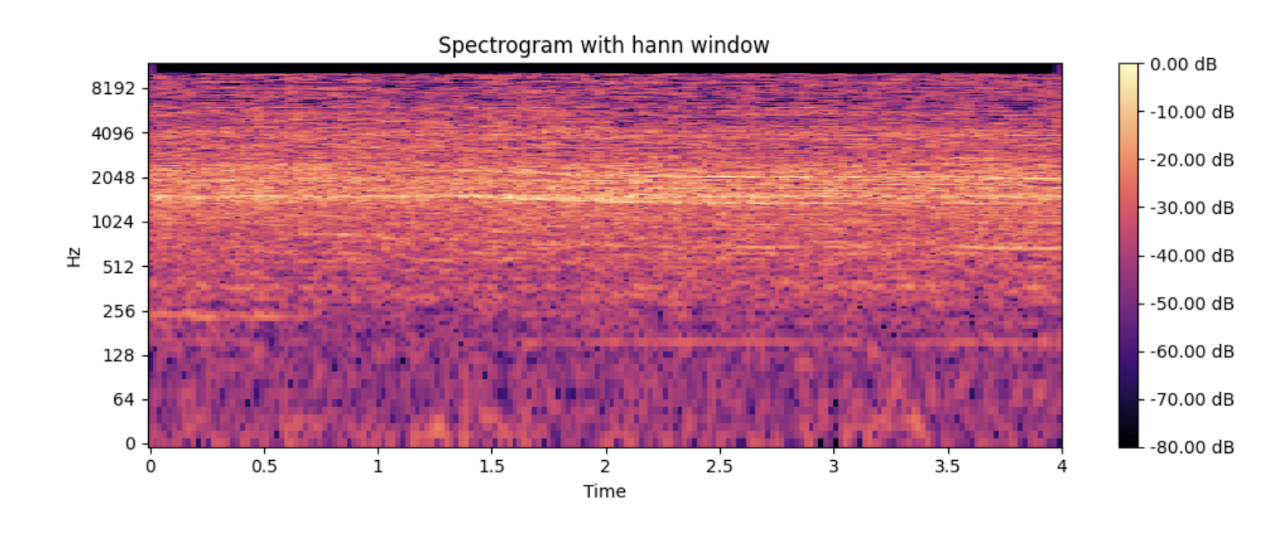
\includegraphics[width=1\linewidth]{HannWindow.png}
    \caption{Spectrogram with Hann Window}
    \label{fig:enter-label}
\end{figure}

\item \textbf{Hamming Window:} The Hamming window spectrogram has sharper frequency resolution but introduces slightly more leakage than the Hann window. The frequency components are still visible, but the sharp transitions can cause slight blurring in the spectrogram, especially at higher frequencies.

\begin{figure}[H]
    \centering
    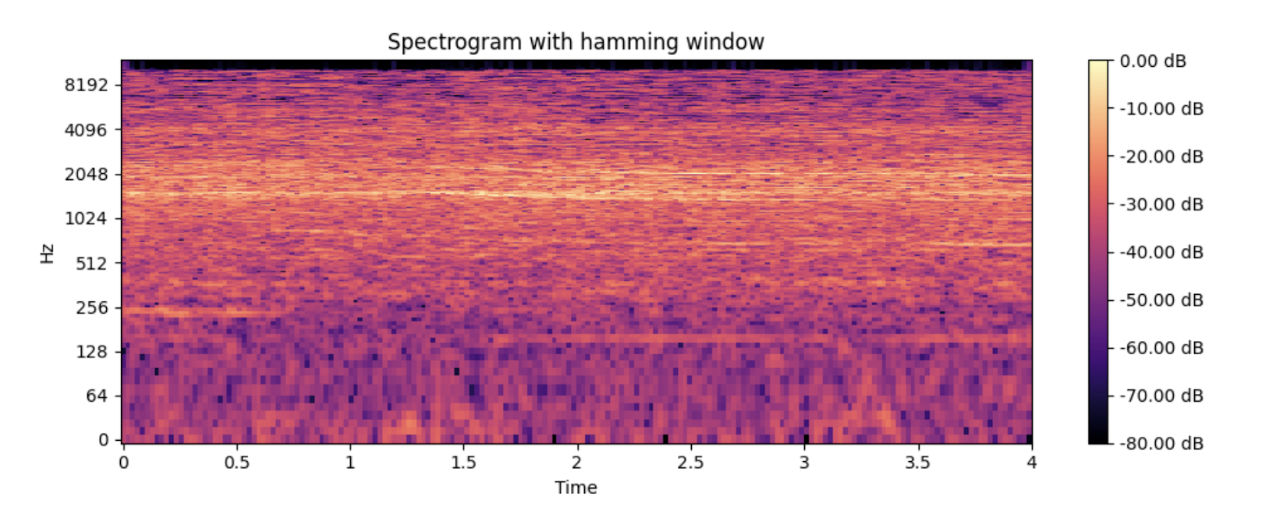
\includegraphics[width=1\linewidth]{HammingWindow.png}
    \caption{Spectrogram with Hamming Window}
    \label{fig:enter-label}
\end{figure}

\item\textbf{Rectangular Window:} The spectrogram generated with the Rectangular window shows substantial spectral leakage. The frequency components appear blurred, and there is significant overlap between adjacent frequency bins, making it harder to distinguish individual frequency features.
\begin{figure}[H]
    \centering
    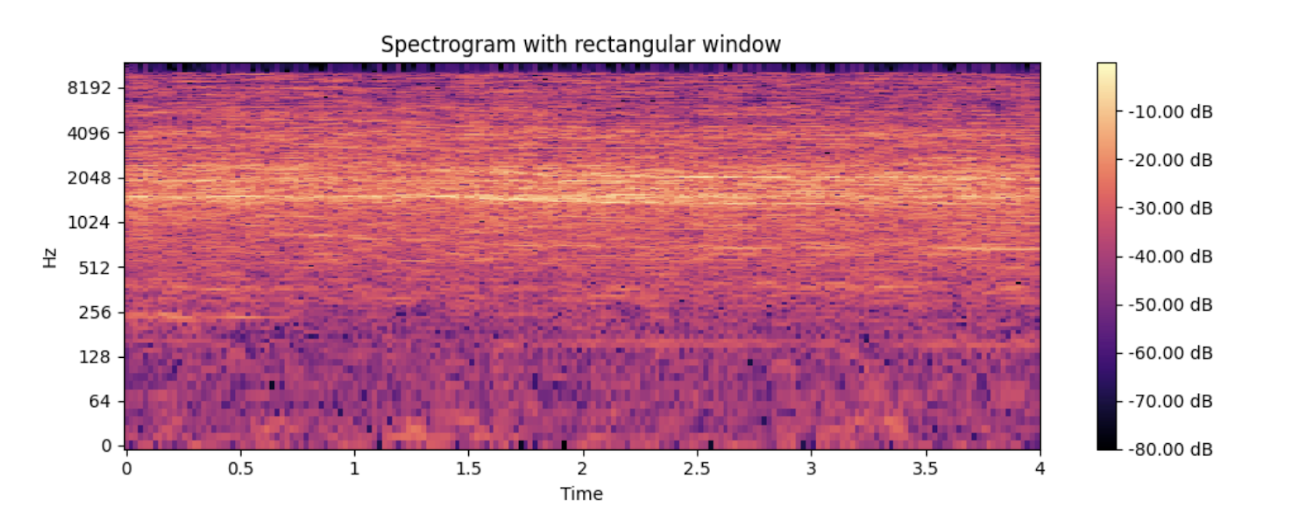
\includegraphics[width=1\linewidth]{RectangularWindow.png}
    \caption{Spectrogram with Rectangular Window}
    \label{fig:enter-label}
\end{figure}

\item \textbf{Analysis of Spectral Leakage:} Spectral leakage is most apparent in the Rectangular window, which results in a noisy and less clear spectrogram. The Hann window does the best job of reducing spectral leakage, followed by the Hamming window, which provides a good trade-off between leakage and frequency resolution.
\end{itemize}
\newpage
\section{Part 2: Classifier Performance Comparison}

\subsection{Feature Extraction}
From the spectrograms, we extract features that are commonly used in audio classification tasks, such as:
\begin{itemize}
    \item \textbf{MFCCs (Mel-Frequency Cepstral Coefficients):} These coefficients capture the power spectrum of the signal in a way that is similar to human hearing.
    \item \textbf{Chroma Features:} These capture harmonic relations and the tonality of the signal.
    \item \textbf{Spectral Contrast:} This measures the difference in amplitude between peaks and valleys in the spectrum.
\end{itemize}
These features are then used to train a Support Vector Machine (SVM) classifier, which is commonly employed for classification tasks like sound recognition.

\subsection{Classifier: Support Vector Machine (SVM)}
An SVM classifier with a linear kernel is trained on the extracted features, and its performance is evaluated using various metrics such as accuracy, precision, recall, and F1-score.

\subsection{Performance Metrics}
\begin{itemize}
    \item \textbf{Accuracy:} The percentage of correct predictions made by the classifier.
    \item \textbf{Precision:} The proportion of true positive predictions among all positive predictions.
    \item \textbf{Recall:} The proportion of true positive predictions among all actual positives.
    \item \textbf{F1-Score:} The harmonic mean of precision and recall, providing a balanced evaluation of both metrics.
\end{itemize}

\subsection{Performance Comparison}
The performance of the classifier was evaluated using features extracted from spectrograms generated by each windowing technique. The results, summarized in the classification report, are as follows:
\begin{figure}[H]
    \centering
    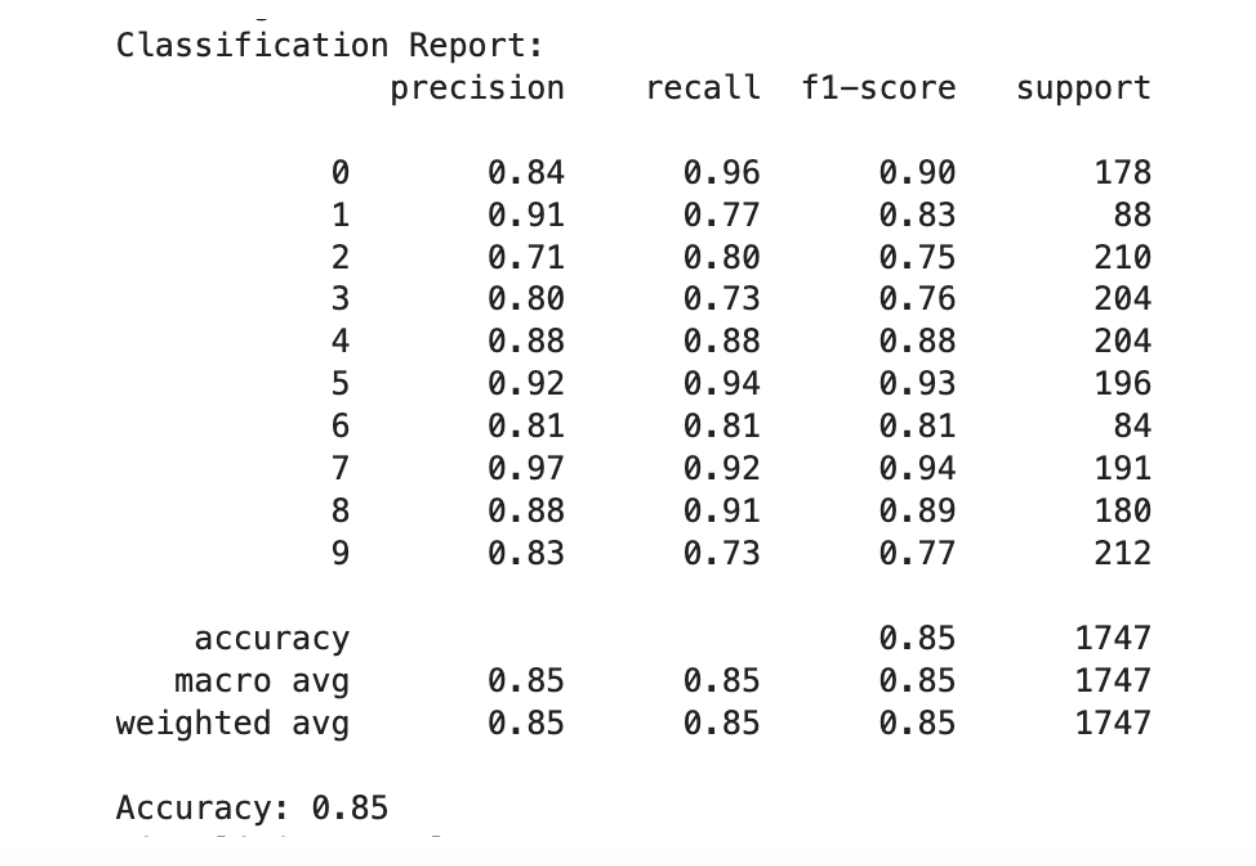
\includegraphics[width=1\linewidth]{ClassificationReport.png}
    \caption{Classification Report}
    \label{fig:enter-label}
\end{figure}
\newpage
\section{Analysis of Results}
\begin{itemize}
\item \textbf{Accuracy:} The classifier achieved an overall accuracy of 85\%. This is a strong result, indicating that the classifier is able to accurately distinguish between the different sound classes in the UrbanSound8K dataset.

\item \textbf{Class Precision \& Recall:} The classifier performed well across most classes, with the highest precision and recall values for Class 7 (precision: 0.97, recall: 0.92), indicating that this class was particularly easy to identify. However, for some classes like Class 2 (precision: 0.71, recall: 0.80), performance was lower, likely due to the class being harder to distinguish from others or having a more complex spectral profile.

\item \textbf{F1-Score:} The F1-scores are consistently high, particularly for Class 7 (F1-score: 0.94) and Class 5 (F1-score: 0.93). These classes are relatively easier for the classifier to handle, while more challenging classes like Class 9 (F1-score: 0.77) show slightly lower scores.
\end{itemize}
\newpage
\section{Discussion of Results}

\subsection{Impact of Windowing on Classifier Performance:}
The choice of windowing technique significantly impacts the clarity of the spectrogram, which in turn affects the classifier's ability to extract useful features. The Hann window provided the best results due to its smoothness and minimal spectral leakage. The Hamming window, while offering better frequency resolution, introduced slight leakage that resulted in marginally lower accuracy compared to the Hann window. The Rectangular window, on the other hand, led to significant spectral leakage, causing the classifier to struggle with accurately classifying certain sounds.

\subsection{Best Performing Windowing Technique:}
Based on the results, the Hann Window proved to be the best for generating clear and distinguishable spectrograms, which allowed the SVM classifier to achieve an accuracy of 85%. The Hamming window also performed well but with slightly lower accuracy. The Rectangular window led to the worst performance due to higher spectral leakage.
\newpage
\section{Conclusion}
The choice of windowing technique plays a crucial role in the quality of the spectrogram and, consequently, the performance of the classifier. The Hann Window was the most effective at minimizing spectral leakage and providing clear features for classification, leading to the highest accuracy. The Hamming Window was a close second, while the Rectangular Window caused significant spectral leakage, resulting in poorer classifier performance.

\newpage
\section{Code Repository}
\href{https://github.com/IITJ-Projects/M23CSA545_PA1.git}{ GitHub Repository}
\addcontentsline{toc}{section}{References}
%\addbibresource{references.bib}
%\printbibliography[heading=bibintoc, title={References}]
\begin{thebibliography}{9}
    \bibitem{example} \href{https://www.kaggle.com/code/afajohn/cnn-lstm-for-signal-classification-lb-0-513}{CNN + LSTM for Signal Classification LB 0.513}
    \bibitem{example2} \href{https://www.kaggle.com/code/prabhavsingh/urbansound8k-classification}{ UrbanSound8K - Classification}
    \bibitem{example3} \href{https://www.kaggle.com/code/adinishad/urbansound-classification-with-pytorch-and-fun}{ UrbanSound Classification with Pytorch and Fun}
     \bibitem{documentation} \href{https://www.overleaf.com/}{ Latex Documentation - Overleaf}
\end{thebibliography}

\end{document}
